\section{Emissions probabilities and coupled future alternatives}
\subsection{Recovered priors and unresolved expert density}
The written emissions constraints are more specific than the initial blocker
assessment implied. Darnell's manuscript and its published successor specify
the cumulative interval as 2022--2100 and describe annual selection of the
nearest SSP CO$_2$ trajectory\cite{darnell}. The prior peak year can occur after
the simulation horizon. The implementation now retains such draws as growing
trajectories through the last simulated year, rather than rejecting valid
prior mass. Ten thousand independent draws contain eight such peaks after 2150.
The starting net emissions, including the documented cement-carbonation
adjustment to Global Carbon Budget 2023, are 40.663 GtCO$_2$ yr$^{-1}$ in 2022.

Only 2.35\% of these prior draws satisfy the 1223 GtCO$_2$ cumulative budget.
The written 50\% and 75\% expert assessments therefore imply substantial
reweighting. They do not specify a unique density, and the baseline requirement
that SSP4-6.0 be the conditional mode above the budget imposes information beyond a single event probability.
To isolate this ambiguity, two explicit alternatives minimize relative entropy
with respect to the empirical sample from the documented prior subject only to the budget-event
probability. If $A$ denotes draws within the budget, $n_A$ its size and $p$ the
imposed probability, the weights are
\begin{equation}
 w_i=\begin{cases}p/n_A,&i\in A,\\
 (1-p)/(n-n_A),&i\notin A.\end{cases}
\end{equation}
This formula follows from Lagrange multipliers and leaves conditional
distributions within each class unchanged. It does not recover the elicited
expert density or the SSP4-6.0 mode. The effective weighted sample sizes are 918
and 417 for $p=0.5$ and 0.75. Changing peak-year rounding to floor or ceiling
changes budget membership for 28 or 21 draws; trapezoidal rather than annual-mean
summation changes 26 memberships. These sensitivities are retained explicitly.

\begin{figure}[htbp]
\centering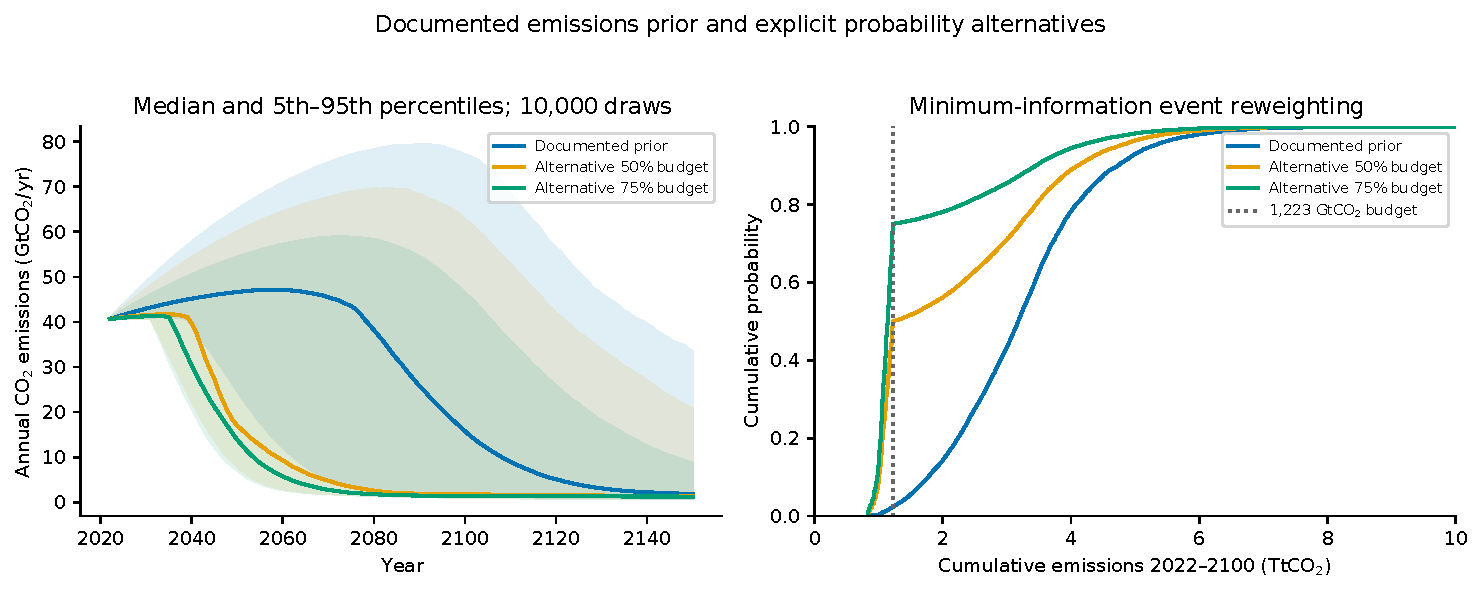
\includegraphics[width=\linewidth]{figures/emissions_probability_alternatives.pdf}
\caption{Documented emissions priors and explicit alternative weighting.
Left: weighted medians and 5th--95th percentiles of annual emissions. Right:
cumulative budget distributions and the 1223 GtCO$_2$ threshold. All distributions
use the same 10,000 independent draws; only their weights differ. The two
reweighted distributions are non-reproductions of the published emissions
posterior.}\label{fig:emissionweights}
\end{figure}

\subsection{Independent SSP inputs and carbon--climate coupling}
The RCMIP protocol 5.1.0 supplies independent exogenous SSP emissions rather than
Wong model outputs\cite{rcmip}. Total global CO$_2$, fossil and industrial
CO$_2$, and land-use CO$_2$ are extracted for six SSPs and linearly interpolated
between supplied annual nodes. Their partition identity closes to
$2.9\times 10^{-14}$ GtCO$_2$ yr$^{-1}$. No extrapolation is needed through 2150.
The interpretation tested here selects, separately each year, the SSP with
smallest absolute total-emissions difference. CEDA non-CO$_2$ forcing from
that scenario is then linearly interpolated between annual nodes. A paired
fixed-SSP2-4.5 calculation measures the consequence of this selection. The
written nearest-trajectory statement alone does not settle all interpolation
and distance conventions.

The future calculation starts from the conditional carbon hindcast and the
accepted climate posterior's physical temperature state in 2021. Carbon
feedback temperature is transformed to the same preindustrial datum used in
the carbon fit. The future CO$_2$ forcing uses $3.7\log_2(C/280)$ W m$^{-2}$;
its difference from the historical CEDA forcing is reported as a restart
discontinuity, without compensating adjustment. The carbon fertilization
parameter is fixed at the independently fitted central value; uncertainty
in this parameter and its dependence on climate parameters are omitted.
The resulting distribution is therefore conditional and cannot stand in for
the target joint posterior.

A balanced conditional sample contains 128 draws on each side of the budget.
Complete accepted climate-posterior rows are paired independently with these
emissions draws. Each probability measure retains its own class weights.
An eight-member pilot with both forcing rules verifies carbon conservation and
compares eight with sixteen coupling substeps per year. The maximum differences
are $1.45\times 10^{-5}$ K in temperature and $3.96\times 10^{-4}$ ppm in CO$_2$;
these checks precede the 256-member calculation. Warming categories use the
annual 2100 temperature relative to 1850--1900, with boundary values assigned
to the lower category exactly as in the publication.

\begin{figure}[htbp]
\centering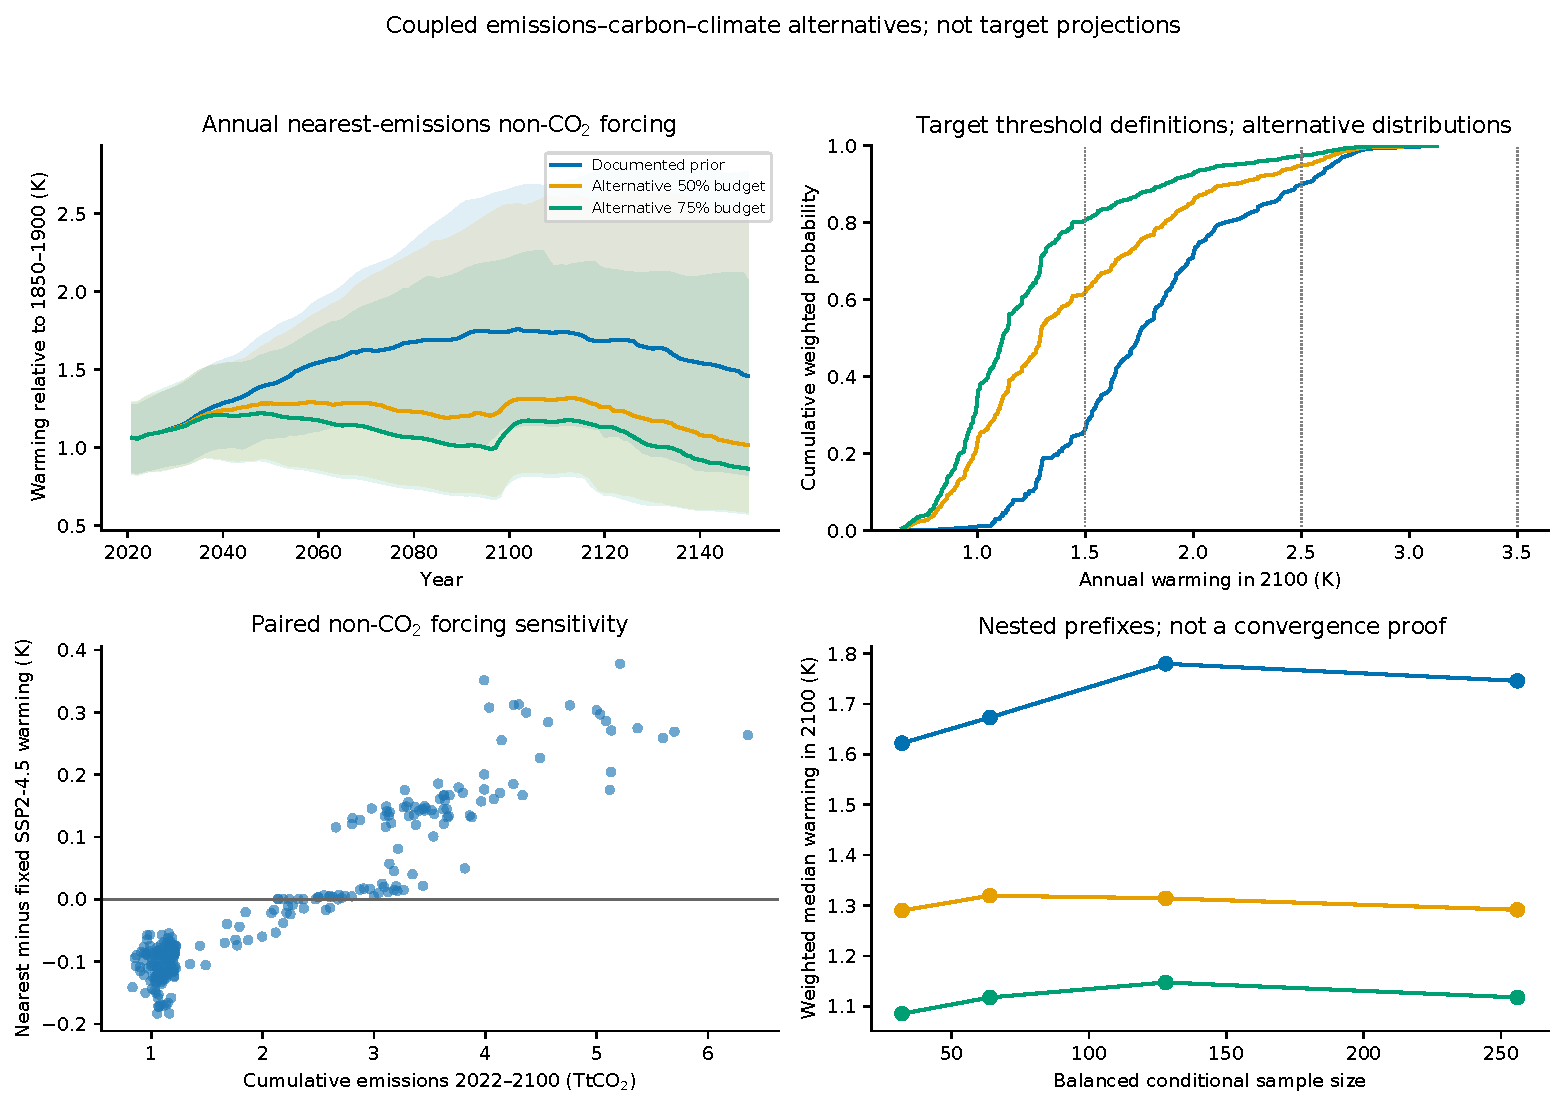
\includegraphics[width=\linewidth]{figures/coupled_emissions_alternatives.pdf}
\caption{Coupled alternative future experiments. Upper left: median and
5th--95th temperature ranges for the three weighting measures. Upper right:
weighted 2100 temperature distributions and the published category boundaries.
Lower left: paired sensitivity to annual nearest-emissions versus fixed-SSP2-4.5
non-CO$_2$ forcing. Lower right: medians for nested balanced sample sizes;
stability of these medians alone is not evidence of tail convergence.
Carbon parameters are conditionally fixed and climate rows are independently
paired, so no panel is a recovered published projection.}\label{fig:coupledfuture}
\end{figure}
\begin{table}[htbp]
\centering\small
\begin{tabular}{lrrrrrrr}
\toprule
Distribution & $T_{.05}$ & $T_{.50}$ & $T_{.95}$ & $P_1$(\%) & $P_2$(\%) & $P_3$(\%) & $P_4$(\%) \\
\midrule
Prior & 1.136 & 1.746 & 2.650 & 26.0 & 63.3 & 10.7 & 0.0 \\
50\% alternative & 0.811 & 1.291 & 2.552 & 61.7 & 32.8 & 5.5 & 0.0 \\
75\% alternative & 0.784 & 1.117 & 2.211 & 80.5 & 16.8 & 2.7 & 0.0 \\
\bottomrule\end{tabular}
\caption{Alternative annual warming in 2100 relative to 1850--1900, in K. Probabilities refer to the four published threshold definitions. The balanced 256-member subsample has distinct weights for each probability measure; it is not the published 5,000-member ensemble.}
\end{table}
The largest paired change in 2100 warming from nearest-scenario versus fixed-SSP2-4.5 non-CO$_2$ forcing is 0.378 K. The restart changes the CO$_2$ forcing by -0.1762 W m$^{-2}$, without compensation. Maximum carbon accounting error is 8.3e-12 Gt C.


No member of this256-member calculation exceeds3.5 K. The zero entry in the
fourth category therefore denotes absence in this finite sample, not proof of
zero probability. A separate tail-stratified emissions experiment is motivated
by this limitation; it preserves empirical prior class masses with explicit
weights rather than changing parameters to create high warming.
\subsection{Recovering the probabilistic-inversion convention}
The cited method of Fuller et al.~\cite{fuller2017} uses the expert assessment
as a likelihood evaluated at the model output. For emissions parameters
$\theta$, prior $p_0(\theta)$, cumulative emissions $C(\theta)$ and expert
density $f$, the resulting density is
\begin{equation}
 p(\theta\mid f)\propto p_0(\theta)f[C(\theta)].
\end{equation}
Consequently, assigning half the expert density below a carbon budget does
not require half the posterior model outputs to fall below that budget.
The earlier event-weighting experiment is a different statistical assumption.

We test four explicit expert-density alternatives. Each assigns half its
mass below $B=1223$ GtCO$_2$, using either a uniform or scaled Beta$(2,2)$
density on $(0,B)$. Above $B$, a shifted gamma density has shape 2 or 4 and
scale $(M-B)/(k-1)$, where $k$ is its shape. Thus its conditional mode is
$M=3263.330$ GtCO$_2$, the independently computed annual SSP4--6.0 sum for
2022--2100. The two documented assessment constraints are respected, but
the density families and shapes are alternatives, not recovered target inputs.
Integration and mode tests verify all four densities.

Reweighting the 10,000 independent prior draws yields posterior budget
probabilities of 4.56--11.31\%, despite the common 50\% assessment mass.
Reweighting the 250 propagated paths gives 4.36--11.05\%; their normalizing
constant differs from the larger prior sample by 2.42--5.22\%. Effective
sample sizes are 65--83 for the propagated paths. Median 2100 warming is
1.78--1.85 K, and unconditional median incremental coastal cost is
0.266--0.277 trillion 2019 USD PPP. These calculations identify a consequential
statistical distinction without identifying the missing target density.

\begin{figure}[htbp]
\centering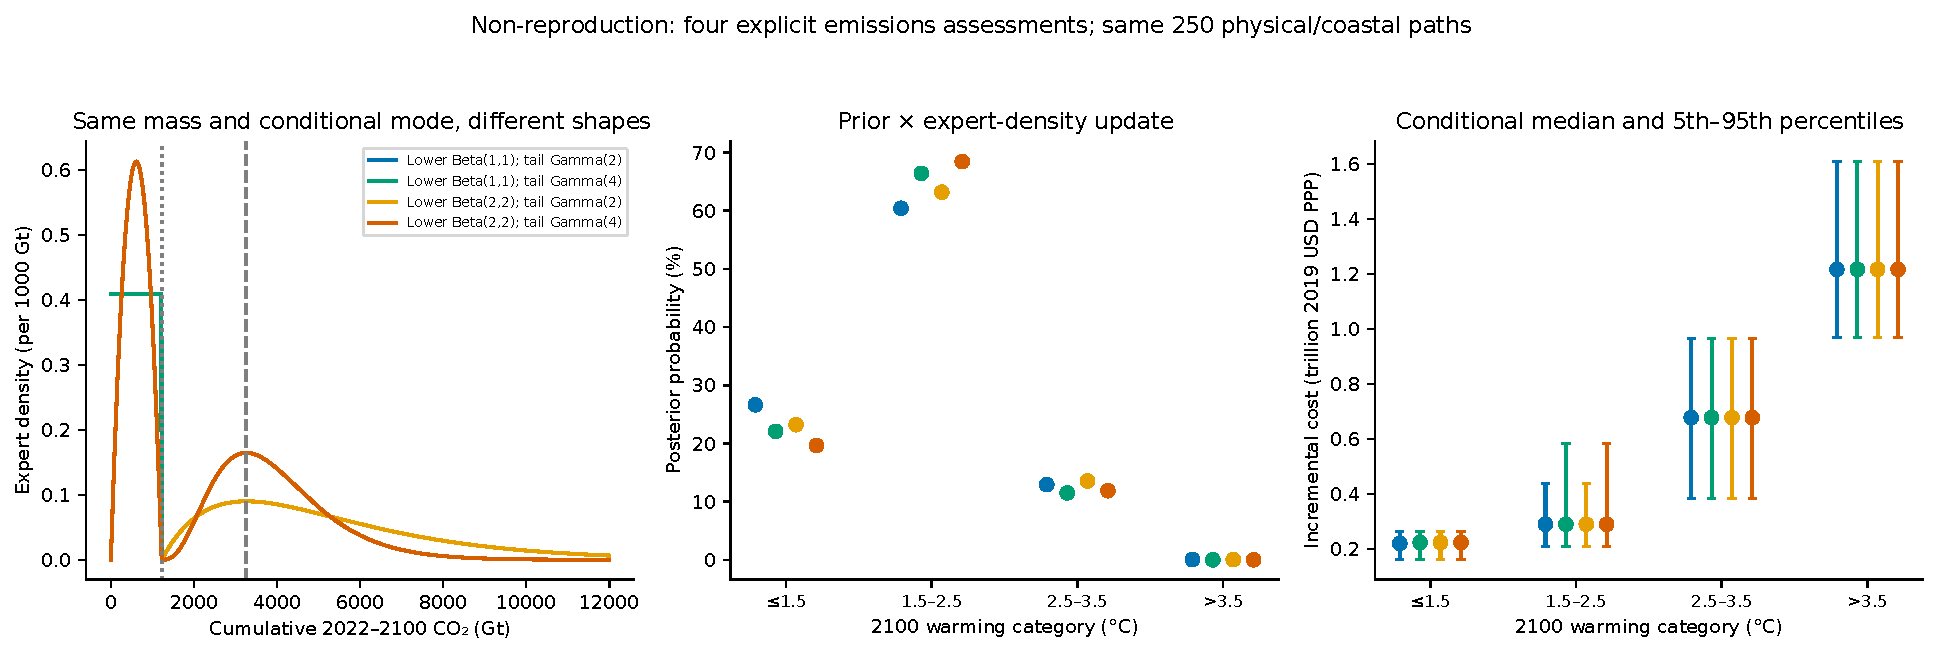
\includegraphics[width=\linewidth]{figures/emissions_inversion_sensitivity.pdf}
\caption{Four explicitly assumed expert densities and their propagation
through the same independent climate, sea-level and coastal calculations.
Left: equal assessment mass below the budget and the same conditional
above-budget mode do not determine a unique density. Middle: warming
probabilities after multiplying the parameter prior by the expert density.
Right: conditional coastal cost medians and 5th--95th order statistics.
Five physical paths remain in the highest warming category; reweighting
does not resolve its tails. All panels are non-reproductions.}
\end{figure}
